%%%%
\section{África}

A poluição do ar ambiental nas cidades dos países em desenvolvimento
guarda algumas similaridades com as cidades dos países desenvolvidos, já que 
ambas possuem algumas fontes poluidoras que são características de meios urbanos, 
tais como, tráfego de veículos automotivos, indústrias, geração de 
eletricidade por usina hidrelétrica ou termelétrica, entre outras. 

No entanto, em cidades de países industrializados tardiamente, soma-se a esta 
poluição, comum a meios urbanos, agravantes decorrentes da má distribuição de renda e da incapacidade do Estado em atender toda a população nas demandas urbanas por infraestrutura. É o caso, por exemplo, da insuficiência de energia para realização de atividades cotidianas, tais como, transporte, iluminação ou alimentação. 
As alternativas frequentemente encontradas pela população destas cidades são: queima da 
biomassa para cozimento de alimentos, uso de querosene para iluminação 
noturna e contínuo uso de frota veicular com tecnologias ultrapassadas
\citep{brauer2012}.

Esses fatores citados acima e a urbanização rápida e descontrolada ocorrida na
última década fazem com que cidades da Ásia, África e Oriente Médio possuam os maiores níveis de poluição do ar ambiental do mundo 
\citep{brauer2012}.

Em 2015, a África contava com $1.186,178$ habitantes, ficando atrás 
apenas da Ásia, que possuía $4.393,296$ habitantes no mesmo ano.%
%Thiago, confira esses números, pois acho que são bilhões. Pode colocar como misto número e potência (e.g. 1,2 bilhões e 4,4 bilhões)
 
A África é o terceiro maior continente em extensão, com área territorial 
de 30 milhões de quilômetros quadrados, abrigando 54 países independentes 
\citep{UN}.

Existe uma barreira natural formada pelo \textbf{Deserto do Saara},
separando norte e sul da África. Separação não só geográfica, como
social, étnica e econômica. 

A África Subsariana \textbf{(SSA)}, localizada ao sul do 
\textbf{Deserto do Saara}, conta com os países mais pobres do mundo, mas que 
nas últimas décadas iniciaram um processo intenso de urbanização \citep{UN}. 
   	
%%%%
\subsection{África Subsariana \textbf{(SSA)}}

A África Subsariana \textbf{(SSA)} é atualmente a região no mundo com a maior 
taxa de transição da população rural - ainda predominante - para cidade
\citep{MONTGOMERY2008}. 

Até 2003, nenhuma cidade da \textbf{SSA} possuía sistemas de monitoramento 
sistemático de poluição do ar. Havia somente medidas esporádicas, realizadas
por universidades, mas que revelaram concentrações de poluentes altíssimas e 
acimas dos recomendados pela Organização Mundial de Saúde \textbf{OMS},
fato esse que levou pesquisadores do mundo inteiro a 
realizarem estudo ambientais no continente \citep{EZZATI2004}. 
Segundo \cite{aboh2009} ainda há pouco estudos de aerossol atmosférico 
em países africanos, mas o interesse da comunidade acadêmica cresceu
nos último anos. Parte deste interesse deriva de sua interferência no clima  do mundo
(radiação, umidade, vento, etc).

Diferentemente dos países industrializados, onde as principais fontes de poluição 
são os setores da industria e do transporte, nos países da \textbf{SSA} a 
queima de biomassa assume a primazia, sendo comum o seu uso no cozimento 
de alimentos, tanto em regiões urbanas quanto rurais \citep{SMITH2004}. 

Estas são algumas características regionais da \textbf{SSA} que ampliam as 
diferenças do perfil de fontes poluidoras do ar comparada com cidades 
de países desenvolvidos: população predominantemente rural,
vias não pavimentadas, altas taxa de crescimento populacional, população jovem,
inexistência de sistemas de monitoramento sistemático e em larga escala do meio 
ambiente, queima de biomassa em residências e comércio para o preparação
de alimentos, entre outros. 

%%%%
\subsection{Algumas Informações Relevante sobre Gana}

Gana situa-se no continente africano, 5 graus a norte do Equador e 
faz fronteira com a Costa do Marfim a oeste, ao norte com Burkina
e a leste com Togo. 

Com clima equatorial, possui praticamente duas estações climáticas:

\begin{itemize}
  \item seca, caracterizada pelo ar seco e pela poeira do harmatão. 
       Começa no meados de Novembro se estende até metade de Março.
 \item chuvosa, começa em Abril e acaba em outubro, tendo maior
       intensidade entre Abril e Julho.
\end{itemize}

Um vento quente e seco provindo de nordeste sopra entre Novembro e Fevereiro 
e é chamado de Harmatão. O Harmatão vem carregado de poeira do 
\textbf{Deserto do Saara} e é a maior fonte de poeira do mundo
\citep{breuning2005}. Análises de modelos receptores realizadas tanto este trabalho quanto em Zheng et al. (201X)%
%verificar a data do artigo
, mostram que ela representa a principal fonte de material particulado detectado em Acra neste período, tanto na fração fina quanto na grossa.

%essa avaliação da meteorologia vai para a parte de discussão, quando for analisar os resultados de modelos receptores. 
%
%Início de meteorologia a transferir

Para avaliação do perfil dos parâmetros meteorológicos locais
utilizou-se dados horários de Setembro de 2006 à Junho de 2008 
coletados na estação meteorológica do aeroporto de Acra 
(\textbf{Kotoka International Airport}) cadastrado na \textbf{NOAA}, 2015 (\textbf{National Oceanic 
and Atmospheric Administration} - United States Department of Commerce)%
%Você está fazendo uma tabela com acrônimos ou siglas. Isso é interessante para eliminar a inserção deles no texto e facilitar compreendê-los aonde quer que apareçam. Veja que corrigi a NOAA, de acordo como eles se referenciam.
%Precisa pinças todos os acrônimos espalhados pelo texto, eliminar o nome por extenso e colocar nesta tabela. Atenção para o ajuste fino da frase quando fizer esta mudança. 
. Esta mantém um banco de dados com parâmetros 
meteorológicos do mundo inteiro, enviados por estações meteorológicas 
cadastradas.

A figura \ref{fg:rosaCompleta}, 
mostra a distribuição de frequência da direção dos ventos bem, como a 
intensidade. Verifica-se que a direção predominante de origem dos ventos de superfície
é de sudoeste. 

\begin{figure}[H]
  \centering
  \includegraphics[width=0.5\textwidth]{../outputs/windRoseNoaaHarvard.pdf}
  \caption{Rosa do ventos entre
           Setembro de 2006 e Junho de 2008. Utilizou-se dados 
           do \textbf{Kotoka International Airport} de Acra 
           \label{fg:rosaCompleta}}
\end{figure}%
%veja que você não está considerando ciclos anuais completos, ou seja, de junho a junho, setembro a setembro. Isso pode introduzir vícios na avaliação do vento local em termos sazonais. Precisamos refletir um pouco como tratar isso. 

No gráfico da figura \ref{fg:rosaCompleta}%
%precisa de legenda. É necessário explicitar se o período do ano é o mesmo
 a observação horária da direção e 
intensidade dos ventos, identifica-se um forte componente regional para o vento local, associável à brisa marinha, com ventos de sul (do oceano) quando o sol encontra-se alto,%
%sol a pino significa sol no zênit, o que ocorre duas vezes ao ano naquela região e uma vez ao ano em SP.
%Precisa colocar um mapa, ou referir-se ao mapa colocado em outro lugar da tese, para que o leitor possa ver que ao sul fica o oceano
 mas deslocando-se à oeste na medida que as horas avançam (deslocamento à direita do sentido do movimento - ação típica do efeito de Coriolis no hemisfério Norte). 

No gráfico de rosa dos ventos mensal \ref{fig:windRose_mensal}
 nota-se 
perceptível diferença entre os dois períodos climáticos, 
pois no Verão temos maior quantidade de radiação solar, fortalecendo a 
formação de brisa marinha e, consequentemente, havendo maior tempo para a velocidade do vento intensificar-se e para processar-se um deslocamento para oeste.%
%Na maior parte do verão Ganha localiza-se no hemisfério sul em termos de padrão global de circulação. Neste período as intensidades de vento são maiores e são menores as frequências de calmarias. No período do inverno Ghana posiciona-se no hemisfério norte em termos da circulação global. Observa-se com isso maior incidência de vento norte (observe-se particularmente o mês de janeiro), com velocidades médias do vento um pouco menores e maior percentual de calmaria. É nesta época que Gana e o Saara situam-se no mesmo sistema de circulação global, ocorrendo o Harmatão. 

\begin{figure}[H]
  \centering
  \includegraphics[width=1\textwidth]{../outputs/windRose_horaria.pdf}
  \caption{ \citep{carslaw2012} \label{fig:windRose_horaria}}%
  %precisa colocar legenda e período a que se refere
\end{figure}

\begin{figure}[H]
  \centering
  \includegraphics[width=1\textwidth]{../outputs/windRose_mensal.pdf}
  \caption{ \citep{carslaw2012} \label{fig:windRose_mensal}}
\end{figure}

Nos meses de ocorrência do Harmatão (inverno), há um pequeno aumento da frequência de ventos de nordeste ao nível do solo (direção do Saara). Mas a maior parte do particulado que este vento transporta passa por Gana 
em altitudes superiores \citep{breuning2005}, interferindo pouco no predomínio da brisa marinha na circulação local.%
%
%Aqui termina o trecho sobre meteorologia que deve ir para a discussão sobre modelos receptores. 

Os últimos dois censos demográficos realizados em Gana datam
de 2000 \citep{ghanacensus2003} e 2010 \citep{ghanacensus2013}. Os
dados resultantes podem ser encontrados no portal de dados abertos
do Governo Federal de Gana \citep{opendataghana}.

A população de Gana em 2000, $18,9$ milhões de habitantes, subiu para $24,7$ 
milhões em 2010, aumento de $30\%$ no intervalo dos dois censos demográficos. 
Sua pirâmide etária, figura \ref{fig:piramedegana}, indica população 
jovem e baixa expectativa média de vida, sendo  pouco maior que 50 anos. %
%a espectativa etária é uma medida bem definida. Você a obteve do mesmo senso demográfico governamental?
%juntei os dois parágrafos para o texto não ficar muito entrecortado.
\begin{figure}[H]
  \centering
  \includegraphics[width=0.5\textwidth]{../outputs/piramide_etaria.pdf}
  \caption{Pirâmide etária Gana plotada com dados do censo 
           demográfico de 2010 \citep{ghanacensus2013} \label{fig:piramedegana}}
\end{figure}

%troquei a ordem do parágrafo abaixo, sobre distribuição da população, para colocá-lo junto do outro que trata da distribução da economia.
Segundo o censo demográfico de 2010, $49\%$ da população está no meio rural e 
$61\%$ no meio urbano, sendo que as mulheres representam $51,2\%$ da população
total.

A economia de Gana, antes essencialmente dominada pela agricultura, 
agora está distribuída entre: industria $19\%$, agricultura $30\%$ 
e serviços $51\%$. Na industria, recebe destaque a fabricação e exportação de aparelhos digitais, 
automóveis e navios. Em termos de matéria primária, há significativa 
exportação de hidrocarbonetos e minerais
 \citep{ghanacensus2013}.%
 %convém apontar os tipos de minerais.
 %juntei os parágrafos pois o assunto pode seguir como continuidade, reduzindo a fragmentação. A referência também é a mesma.
 

O produto interno bruto (PIB) per capita anual de Gana em 2010 foi
de \$ 1.323,09 USD e, apenas como uma base de comparação, no Brasil foi de \$ 11.124,09 USD.%
%em termos de comparação, se for fácil, seria mais forte colocar a média mundial também.
O gráfico da figura \ref{fg:pib} apresenta o \textbf{PIB} de Gana e do Brasil 
calculado pelo Banco Mundial \citep{bancomundial}.

\begin{figure}[H]
\begin{center}
  \includegraphics[width=0.5\textwidth]{../outputs/PIBGhanaBrazil.pdf}
  \caption{\textbf{PIB} do Brasil e de Gana. Plotado com dados do 
           Banco Mundial \citep{bancomundial} \label{fg:pib}}
\end{center}
\end{figure}

A responsabilidade do controle, fiscalização e monitoramento das 
atividades poluídoras em Gana é realizado pela 
\textbf{Ghana Environmental Protection Agency (EPA Ghana)}, que é 
hierarquicamente subordinada ao 
\textbf{Ministério de Meio Ambiente, Ciência, Tecnologia e Inovação} do 
Governo Federal de Gana.

%%%%
\subsection{Região Metropolitana de Acra \textbf{(RMA)}}

Acra é uma cidade litorânea e é a capital de Gana. Está localizada 
no Golfo da Guiné tendo área total de mais de  $2500 km^2$, com elevações que 
variam de 0 até 60 metros do nível do mar \citep{ARKU2008}.

A Região Metropolitana de Acra \textbf{(RMA)} agrega outras 9 cidades e conta com uma população total de 4 milhões de habitantes (2010). 
Com economia baseada majoritariamente na industria e em serviços, 
$90,5\%$ da população está alocada em área urbana \citep{ghanacensus2013}.

Em 2010, havia aproximadamente 1000 fazendas urbanas com produção de vegetais e
frutas para consumo local da \textbf{(RMA)}. Em geral, as irrigações nessas plantações
são feitas por água não tratada, provinda de córregos locais. 
Altos índices de metais pesados (Fe, Mn, Cu, Zn, Pb, Ni, Cr, Cd, Co)
são encontrados nos alimentos produzidos nessas fazendas, pois resíduos
residências são despejados diretamente nesses córregos \citep{lente2014}.

A densidade populacional em \textbf{(RMA)} é de 1205 $habitantes/km^2$, 
aproximadamente a metade dos 2476 $habitantes/km^2$ que temos na Região Metropolitana de São Paulo \textbf{(RMSP)} 
 \citep{ibge2011}. 

\textbf{Driver and Vehicle Licensing Authority (DVLA)} é o
departamento do governo de Gana que regula e fiscaliza veículos, registrando que em 2009 Gana contava com 1,12 milhões de veículos legais. 
A tabela \ref{table:dvla} mostra que a frota dobrou em 9 anos.
Ressalta-se que além da frota legalizada, é grande o número de veículos circulantes, envelhecidos e não registrados. 

\begin{table}[H]
 \centering
  \begin{tabular}{rr}
  \hline
  Ano & Veículos Registrados \\ 
  \hline
  2000 & 511.083 \\ 
  2001 & 567.780 \\ 
  2002 & 613.153 \\ 
  2003 & 643.824 \\ 
  2004 & 703.372 \\ 
  2005 & 767.067 \\ 
  2006 & 841.314 \\ 
  2007 & 841.314 \\ 
  2008 & 1.033.140 \\ 
  2009 & 1.128.138 \\ 
  \hline
  \end{tabular}
  \caption{Frota veícular de Gana \citep{dvla} \label{table:dvla}}
\end{table}
%
%qual é a frota de Acra?
Segundo a EPA-GH \citep{epa2015} as fontes de poluição do ar ambiental 
majoritárias em Acra são:

\begin{itemize}
 \item Emissões veiculares, principalmente aqueles antigos e sem 
       manutenção;
 \item Emissões industriais;
 \item Queima de lixo e outros materiais a céu aberto;
 \item Poeira de ressuspensão de solo, pois há muitas vias ainda não pavimentadas;
 \item Poeira carregada por vento seco do \textbf{Deserto do Saara}, o Harmatão.
\end{itemize}

Acra é mundialmente conhecida por receber ilegalmente lixo 
eletrônico dos países desenvolvidos, que são impropriamente derretidos, especialmente para a obtenção de cobre pela população local. 
O depósito de lixo eletrônico, conhecido como \textbf{e-waste}, 
fica no bairro \textbf{Agbogbloshie}, apenas $4 km$ a sudoeste de \textbf{Nima}, local que analisamos neste experimento
\citep{asampong2015}.

\begin{figure}[H]
  \centering
  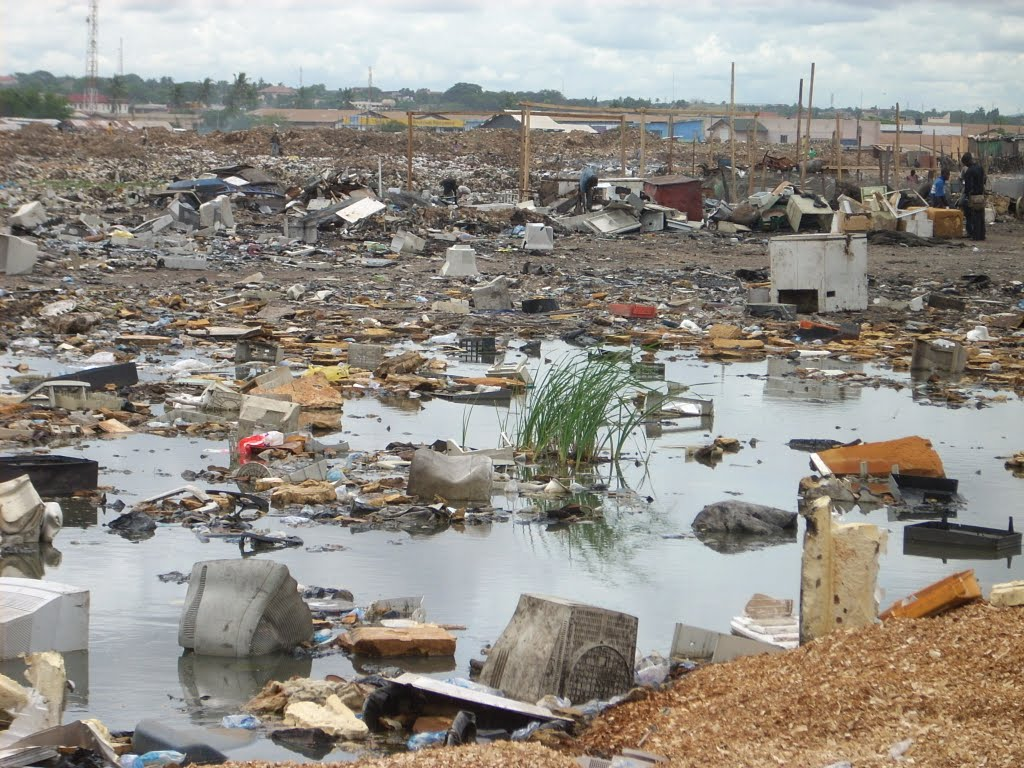
\includegraphics[width=0.5\textwidth]{../inputs/images/ewaste_jack_caravano.jpg}
  \caption{Foto do bairro de Agbogbloshie em Acra. Autorizado por Jack Caravanos, 
           Professor da \textbf{School of Public Health} em \textbf{Hunter College, CUNY}
           Nova Iorque, Estado Unidos da América. \label{fig:ewaste}}
\end{figure}

%%%%
\subsection{Nima}

Nima é um dos bairros mais pobres de Acra. É formada de assentamentos não 
planejados, compostos principalmente de migrantes das partes rurais e 
imigrantes de países vizinhos que buscam oportunidades de empregos na capital. 
Com moradias extremamente improvisadas, carece de sistema tratamento de esgoto, 
fornecimento de água potável e eletricidade. 

É conhecida localmente por uma feira de comidas típicas permanentemente 
instalada na região (\textbf{Nima Market}), que é inclusive visitada por turistas.
Com população de origem de diversas partes de Gana, Nima possui 
alta diversidade cultural e religiosa.

O principal meio de transporte dos trabalhadores de Nima para a zona industrial
e de serviços de Acra é feito por vans. 
Muitas vias não são pavimentadas e a intensa movimentação de veículos causa 
levantamento de poeira do solo.

O carvão e a lenha são bastante empregados como fontes de energia para preparação de 
alimentos. A figura \ref{fig:nima} mostra imagens de áreas de cozimento típicas no bairro.

\begin{figure}[H]
  \centering
    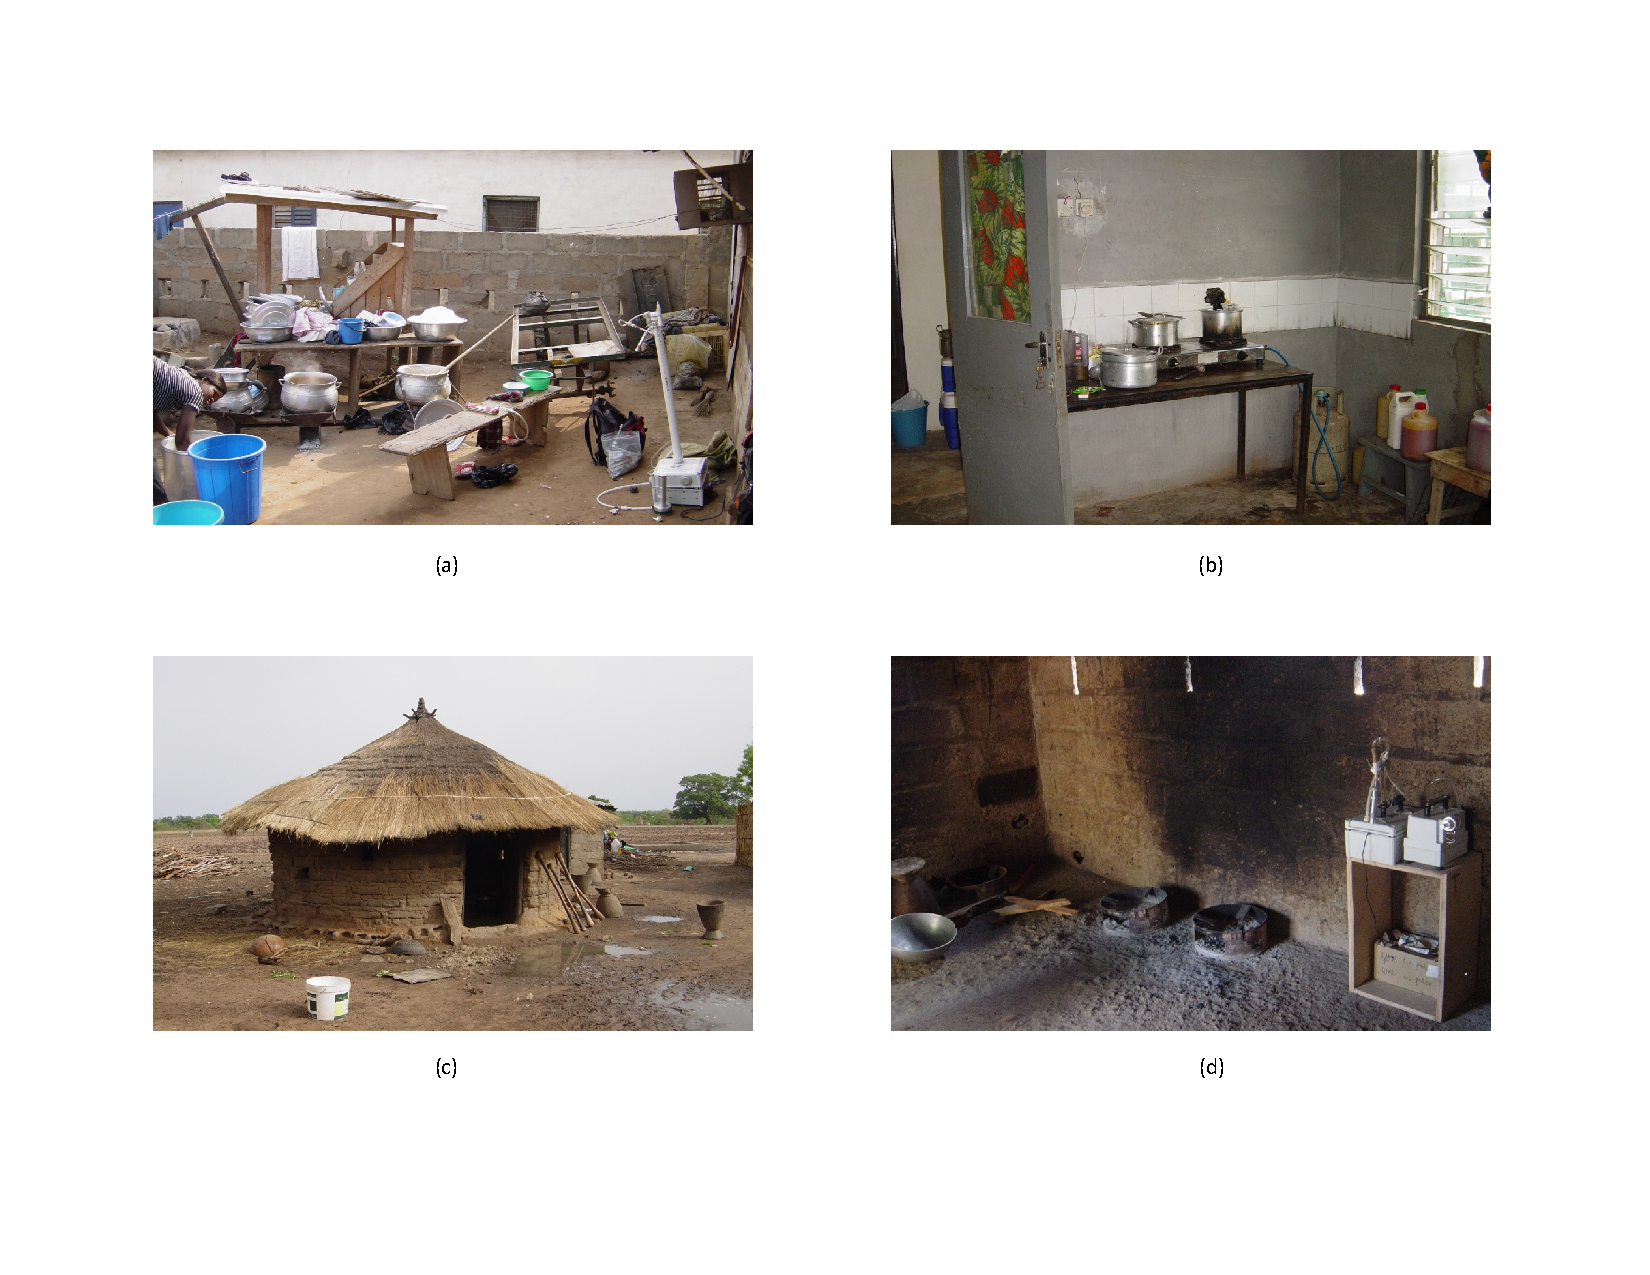
\includegraphics[width=0.7\textwidth]{../inputs/images/zheng/nima.pdf}
    \caption{Fotos de residências de Nima, por Raphael Arku \label{fig:nima}}
\end{figure}%
%precisa recortar a figura para ficar somente com a e b. As imagens de baixo (c e d)são imagens de cozinhas rurais.
